%
% ortho.tex -- Orthogonale
%
% (c) 2019 Prof Dr Andreas Müller, Hochschule Rapperswil
%
\documentclass[tikz]{standalone}
\usepackage{amsmath}
\usepackage{times}
\usepackage{txfonts}
\usepackage{pgfplots}
\usepackage{csvsimple}
\usetikzlibrary{arrows,intersections,math}
\begin{document}
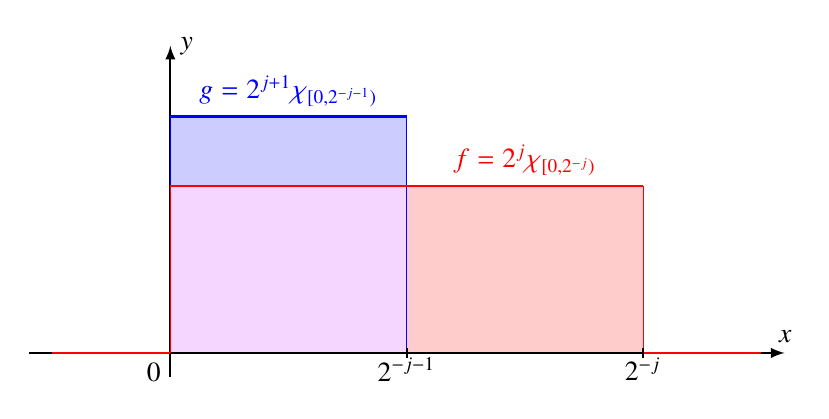
\begin{tikzpicture}[>=latex,scale=3]

\definecolor{pink}{rgb}{0.8,0.2,1}

\fill[color=blue!20] (0,0)--(1,0)--(1,1)--(0,1)--cycle;
\fill[color=red!20] (1,0)--(2,0)--(2,{1/sqrt(2)})--(1,{1/sqrt(2)})--cycle;
\fill[color=pink!20] (0,0)--(1,0)--(1,{1/sqrt(2)})--(0,{1/sqrt(2)})--cycle;

\draw[->,line width=0.7pt] (-0.6,0)--(2.6,0) coordinate[label={$x$}];
\draw[->,line width=0.7pt] (0,-0.1)--(0,1.3) coordinate[label={right:$y$}];

\draw[color=blue,line width=1pt] (0,1)--(1,1);
\draw[color=blue,line width=0.1pt] (0,0)--(0,1);
\draw[color=blue,line width=0.1pt] (1,0)--(1,1);

\draw[color=red,line width=1pt] (-0.5,0)--(0,0);
\draw[color=red,line width=0.1pt] (0,0)--(0,{1/sqrt(2)});
\draw[color=red,line width=1pt] (0,{1/sqrt(2)})--(2,{1/sqrt(2)});
\draw[color=red,line width=0.1pt] (2,0)--(2,{1/sqrt(2)});
\draw[color=red,line width=1pt] (2,0)--(2.5,0);

\node[color=blue] at (0.5,1) [above] {$g=2^{j+1}\chi_{[0,2^{-j-1})}$};
\node[color=red] at (1.5,{1/sqrt(2)}) [above] {$f=2^j\chi_{[0,2^{-j})}$};

\def\s{-0.02};

\draw[line width=0.7pt] (1,-\s)--(1,\s);
\draw[line width=0.7pt] (2,-\s)--(2,\s);

\node at (1,-\s) [below] {$2^{-j-1}$};
\node at (2,-\s) [below] {$2^{-j}$};
\node at (0,0) [below left] {$0$};

\end{tikzpicture}
\end{document}

